\documentclass[tikz,border=12pt]{standalone}
\usepackage{amsmath}
\definecolor{bgcol}{HTML}{171D2B}
\definecolor{accent}{HTML}{F7B538}
\begin{document}
\pagecolor{bgcol}
\color{white}
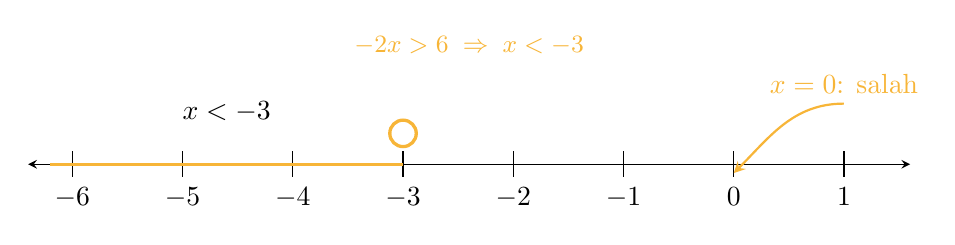
\begin{tikzpicture}[>=stealth, scale=1.4]
  \draw[<->] (-6.4,0) -- (1.6,0);
  \foreach \x in {-6,-5,...,1}
    \draw (\x,0.12) -- (\x,-0.12) node[below] {$\x$};
  \draw[very thick, accent] (-6.2,0) -- (-3,0);
  \draw[very thick, accent] (-3,0.28) circle (0.12);
  \node[above] at (-4.6,0.3) {$x < -3$};
  \draw[->, accent, thick]
    (1.0,0.55) node[above] {$x = 0$: salah}
    to[out=180,in=45] (0,-0.08);
  \node[above, accent] at (-2.4,0.9) {\small $-2x > 6 \;\Rightarrow\; x < -3$};
\end{tikzpicture}
\end{document}
